%!TEX root = thesis.tex

\chapter{Conceptual Design of a TinyMLOps Ecosystem}
\label{chp:Framework}

Building upon the systematic literature review in Chapter~\ref{chp:Research_Results}, which identified critical gaps in operationalizing \gls{ml} on resource-constrained edge devices, this chapter introduces the conceptual design of a novel, integrated ecosystem for autonomous \gls{tinymlops}. This ecosystem is architected to address the challenges of managing the \gls{ml} model lifecycle directly on edge hardware with minimal reliance on centralized infrastructure, while also providing pathways for optional, synergistic server-side support. The ecosystem comprises two primary components: (i) \gls{tinylcm}, an on-device framework engineered for autonomous \gls{ml} model execution, monitoring, and adaptation; and (ii) TinySphere, a server-side platform designed to provide enhanced \gls{mlops} capabilities, including model validation, fleet management, and advanced analytics, specifically tailored to the nuances of \gls{tinyml} deployments.

~\\
\vfill
\minitoc
\clearpage

\section{Motivation and Design Rationale}
\label{sec:framework_motivation_rationale}

Deploying and sustainably operating \gls{ml} models on severely resource-constrained edge devices, such as \gls{mcu} and low-power \gls{sbc}, presents distinct challenges. Traditional \gls{mlops} paradigms, primarily designed for cloud environments with abundant resources, do not adequately address these specific edge-related issues \cite{lerouxTinyMLOpsOperationalChallenges2022a, szydloManagementTinyMLEnabled2024}.

\subsection{Revisiting Research Gaps and Limitations}
\label{ssec:framework_revisiting_gaps}

The findings from Chapter~\ref{chp:Research_Results} (particularly Sections~\ref{sec:RQ1_Results_SystemArchitecture} and \ref{sec:RQ2_Results_Frameworks}) indicate a rapidly evolving yet fragmented \gls{tinyml} operations landscape. Despite significant progress in model compression, on-device inference optimization, and specialized hardware, a cohesive, end-to-end framework for \textit{autonomous} on-device \gls{lcm} is still a critical unmet need.

Many contemporary approaches, even those targeting edge deployment, rely considerably on cloud infrastructure for \gls{mlops} tasks such as continuous model monitoring, retraining, and deploying updated models \cite{kreuzbergerMachineLearningOperations2023, antoniniTinyMLOpsFrameworkOrchestrating2022}. This dependency curtails the operational autonomy of edge devices. Consequently, it poses significant limitations for applications in environments with intermittent, unreliable, or non-existent connectivity—a common characteristic in numerous \gls{tinyml} use cases, such as the Mars rover scenario motivating this thesis.

Furthermore, existing platforms, while powerful within their specific domains, often do not meet the holistic requirements for managing adaptive, autonomous fleets of devices. For instance, platforms such as Edge Impulse provide robust support for the initial development, optimization, and deployment pipeline of \gls{tinyml} models \cite{banburyEdgeImpulseMLOps2023}. However, their primary focus is less on continuous, autonomous on-device adaptation of deployed models or the operational management of numerous, independently evolving devices.

Similarly, generic \gls{mlops} tools like MLflow offer strong capabilities for experiment tracking, model versioning, and deployment in server-based settings \cite{johnMLOpsFrameworkMaturity2021}. Yet, they are not inherently designed for the specific nuances of the \gls{tinyml} context. These nuances include extreme resource constraints (memory, power, computation), the imperative for on-device intelligence, and the need for resilient interaction with device-specific lifecycle processes.

The literature analysis (Chapter~\ref{chp:Research_Results}) also revealed that the integration of comprehensive device management within dedicated \gls{tinymlops} frameworks is still at a nascent stage; this feature, noted as beneficial in systems like SensiX++ \cite{minSensiXBringingMLOps2023}, is not yet widely incorporated. This confluence of observations underscores a pressing need: a server-side \gls{mlops} platform purposefully architected for the \gls{tinyml} paradigm. Such a platform must understand, interact with, and augment autonomous on-device operations, rather than merely adapting existing cloud-centric tools.

\subsection{Objectives and Core Tenets for the Ecosystem}
\label{ssec:framework_derived_objectives}

The aforementioned research gaps and limitations directly inform the primary objectives and guiding architectural principles for the proposed \gls{tinymlops} ecosystem. The overarching goal is to empower resource-constrained edge devices with genuine operational autonomy throughout the entire \gls{ml} model lifecycle. This entails enabling devices to independently monitor their operational context, detect and adapt to changes such as concept drift, manage their own state, and continue functioning effectively even without external communication. Concurrently, the ecosystem provides an optional, yet deeply synergistic, server-side infrastructure (TinySphere) for enhanced management, centralized validation, fleet oversight, and advanced analytics when connectivity and resources permit. This dual-component architecture aims for a pragmatic balance between maximal on-device self-sufficiency and the recognized benefits of centralized \gls{mlops} capabilities.

The ecosystem's design philosophy is ``autonomy-first.'' The on-device framework, \gls{tinylcm}, is engineered as the primary locus of intelligence, performing all critical lifecycle functions locally. These include continuous, label-agnostic monitoring for concept drift, on-device model adaptation in response to detected changes, and robust local state management, including versioning and rollback facilities. The server-side platform, TinySphere, is conceived as an optional, value-adding component, designed to ingest operational data and events from \gls{tinylcm} instances. It offers advanced analytical capabilities, facilitates external validation of on-device adaptations, and provides comprehensive fleet management functionalities.

In terms of architectural patterns, informed by the findings in Chapter~\ref{chp:Research_Results} (Section~\ref{sec:RQ1_Results_SystemArchitecture}), the proposed ecosystem strategically combines established paradigms. For the on-device \gls{tinylcm} framework, a \textit{data-centric pipeline architecture} is adopted. This choice is motivated by its prevalence in existing \gls{tinyml} systems (as identified in Section~\ref{ssec:SystemArchitectureResults}) and its inherent suitability for efficiently processing sequential data streams on edge devices, facilitating modularity and a clear flow of operations from feature extraction through drift detection and adaptation. For the interaction between \gls{tinylcm} and TinySphere, an \textit{client-server model} is employed. While a client-server dependency might seem to contradict the autonomy goal, this pattern is implemented such that \gls{tinylcm} functions independently, attempting to engage with TinySphere only when network connectivity is available and interaction is beneficial (e.g., for data offloading or validation). This server-side interaction is considered crucial for realizing a full spectrum of \gls{mlops} capabilities. The design of TinySphere itself directly responds to the lack (identified in Section~\ref{ssec:framework_revisiting_gaps}) of TinyML-centric \gls{mlops} platforms supporting such a hybrid autonomous-collaborative operational model.

\section{System Requirements and Architectural Vision}
\label{sec:framework_requirements_vision}

To translate the objectives and design rationale into a concrete system, this section establishes functional and non-functional requirements. These requirements are directly informed by the preceding literature analysis (Chapter~\ref{chp:Research_Results}), the overarching goal of enabling autonomous on-device \gls{ml} \gls{lcm}, and the operational challenges exemplified by the Mars rover case study which serves as a guiding scenario. Subsequently, a high-level architectural vision for the complete ecosystem, illustrating the interplay between its on-device and server-side components, is presented.

\subsection{Functional and Non-Functional Requirements}
\label{ssec:framework_requirements}

The functional requirements (FR) define the core capabilities that the ecosystem must deliver to achieve its objectives. The non-functional requirements (NFR) specify the essential quality attributes that govern its performance, usability, and suitability for operation in resource-constrained environments. These are summarized in Table~\ref{tab:functional_requirements} and Table~\ref{tab:non_functional_requirements_v2}.

\begin{table}[htbp]
    \caption[Functional Requirements for the TinyMLOps Ecosystem]{Functional Requirements for the TinyMLOps Ecosystem.}
    \label{tab:functional_requirements}
    \begin{tabularx}{\linewidth}{@{}lX@{}}
        \opentableheader
        \hl{ID} & \hl{Description} \\
        \closetableheader
        FR1 & \textit{Autonomous On-Device Drift Detection:} The on-device component must be capable of continuously monitoring input data characteristics and/or model behavior to detect potential concept drift using proxy metrics, without requiring real-time ground truth labels. \\
        FR2 & \textit{Informed On-Device Model Adaptation:} Upon detection of a potential drift, \gls{tinylcm} must provide mechanisms for immediate, yet cautious, on-device adaptation of the deployed \gls{ml} model. \\
        FR3 & \textit{Robust On-Device State Management:} \gls{tinylcm} must implement robust state management, including versioning of models and relevant operational states, to enable rollbacks to previous stable states if an adaptation proves detrimental or an error occurs. \\
        FR4 & \textit{Opportunistic Synchronization:} \gls{tinylcm} must support optional and opportunistic synchronization of its state, operational logs, detected drift events, and (pseudo-)labeled data with a designated server-side component. \\
        FR5 & \textit{Centralized Monitoring and Fleet Management:} TinySphere should provide capabilities for the centralized monitoring of a fleet of deployed devices, offering insights into their operational status, model performance, and encountered drift phenomena. \\
        FR6 & \textit{Flexible Operational Modes:} The ecosystem must support distinct operational modes, ranging from purely autonomous on-device operation to fully server-assisted adaptive learning, configurable per device or application. \\
        \bottomrule
    \end{tabularx}
\end{table}

\begin{table}[htbp]
    \caption[Non-Functional Requirements for the TinyMLOps Ecosystem]{Non-Functional Requirements for the TinyMLOps Ecosystem.}
    \label{tab:non_functional_requirements_v2}
    \begin{tabularx}{\linewidth}{@{}lX@{}}
        \opentableheader
        \hl{ID} & \hl{Description} \\
        \closetableheader
        NFR1 & \textit{Resource Efficiency:} All on-device components must be optimized for minimal consumption of memory (RAM and flash), CPU cycles, and power, suitable for deployment on \glspl{mcu} and low-power \glspl{sbc}. \\ % Changed to \glspl
        NFR2 & \textit{Modularity and Extensibility:} Both \gls{tinylcm} and TinySphere must be designed with a modular architecture, allowing for straightforward extension or replacement of individual components (e.g., drift detection algorithms, classifiers, server-side analysis modules). \\
        NFR3 & \textit{Scalability:} The server-side platform must be designed to handle data and communication from a potentially large number of connected edge devices. \\
        NFR4 & \textit{Reliability and Fault Tolerance:} The on-device framework must operate reliably under adverse conditions, and synchronization mechanisms must be fault-tolerant, capable of resuming after interruptions. \\
        NFR5 & \textit{Configurability:} Key parameters of \gls{tinylcm}, such as drift detection sensitivity, adaptation strategies, and synchronization policies, must be configurable to suit diverse application needs and hardware capabilities. \\
        \bottomrule
    \end{tabularx}
\end{table}

\subsection{Overall Ecosystem Architecture}
\label{ssec:framework_overall_architecture}

The proposed ecosystem is architecturally conceived as a synergistic pairing of the on-device \gls{tinylcm} framework and the server-side TinySphere platform. \gls{tinylcm} functions as an intelligent, autonomous agent on each edge device, responsible for local \gls{ml} model management. TinySphere serves as an optional, centralized hub, augmenting these on-device capabilities by providing robust backend support for \gls{mlops} processes impractical or overly resource-intensive for individual constrained devices. These server-side functions include comprehensive data aggregation, advanced analytics, human-in-the-loop validation workflows, and fleet-wide operational oversight.

Figure~\ref{fig:ecosystem_context_diagram} presents a high-level system context diagram, illustrating the primary ecosystem components and their interactions. On the edge device, \gls{tinylcm} interfaces with local sensors (e.g., a camera) and the deployed \gls{ml} model. It autonomously executes tasks such as feature processing, inference, drift detection, and model adaptation. A critical sub-component, the \texttt{SyncClient}, manages opportunistic, typically HTTPS-based, communication with the TinySphere API. Through this client, \gls{tinylcm} can transmit packaged data—including drift events, operational metrics, samples quarantined during adaptation, and logs—and receive validated feedback or model updates from the server.

TinySphere, on the server side, processes these incoming data packages. It utilizes a relational database (e.g., PostgreSQL) for structured metadata and an object storage solution (e.g., MinIO) for larger artifacts such as images or extensive logs. TinySphere can leverage external \gls{mlops} tools like MLflow for functionalities such as model registry and experiment tracking, thereby integrating established practices. A web dashboard provides \gls{ml} engineers and data scientists with interfaces for monitoring device fleets, analyzing drift events, managing models, and potentially initiating validation workflows.

\begin{figure}[htbp]
    \centering
    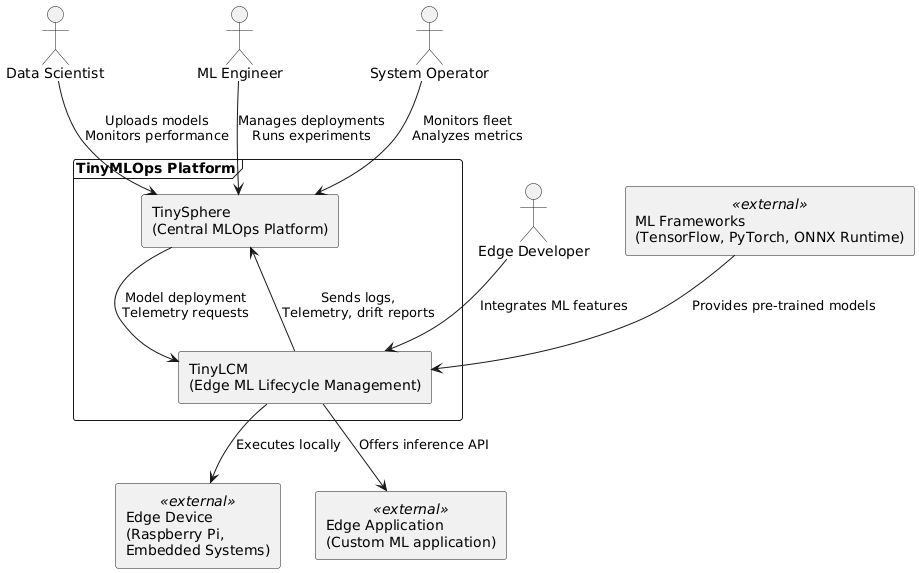
\includegraphics[width=0.75\textwidth]{figs/framework/system-context.png}
    \caption[High-Level System Context Diagram of the TinyMLOps Ecosystem]{High-Level System Context Diagram of the TinyMLOps Ecosystem, illustrating the interaction between Edge Devices (running \gls{tinylcm}) and the TinySphere Server.}
    \label{fig:ecosystem_context_diagram}
\end{figure}

A fundamental characteristic of this architecture is that \gls{tinylcm} is engineered for autonomous on-device \gls{lcm}, even in the complete and prolonged absence of TinySphere. Integration with TinySphere is an enhancement, significantly augmenting edge device capabilities by connecting them to a broader, managed TinyML deployment when circumstances permit. This directly supports FR6, allowing deployments to scale from fully disconnected local autonomy to a comprehensively managed, server-assisted system.


\section{TinyLCM On-Device Framework for Autonomous Lifecycle Management}
\label{sec:tinylcm_detailed_design}

At the core lies \gls{tinylcm}, the on-device framework specifically engineered to endow resource-constrained edge devices with the intelligence and mechanisms required for autonomous \gls{ml} model management. Designed with Python for broad compatibility and leveraging \gls{tfl} for efficient inference, \gls{tinylcm} embodies the ``autonomy-first'' principle of the ecosystem. Its architecture is modular and pipeline-driven, optimized at multiple levels to operate within the severe limitations of hardware such as MCUs and low-power \glspl{sbc}. This section provides a detailed exposition of \gls{tinylcm}'s architectural blueprint, its constituent components, the foundational algorithms for its autonomous drift detection and adaptation capabilities, and the array of resource-optimization tactics employed in its implementation.

\subsection{Architectural Blueprint and Core Components}
\label{ssec:tinylcm_architecture_blueprint}

The internal architecture of \gls{tinylcm} is structured as a pipeline of interconnected, modular components, as illustrated in the component diagram in Figure~\ref{fig:tinylcm_component_diagram}. This design promotes a clear and efficient flow of data and control, from input processing through inference, monitoring, drift detection, and on-device adaptation.

\begin{figure}[htbp]
    \centering
    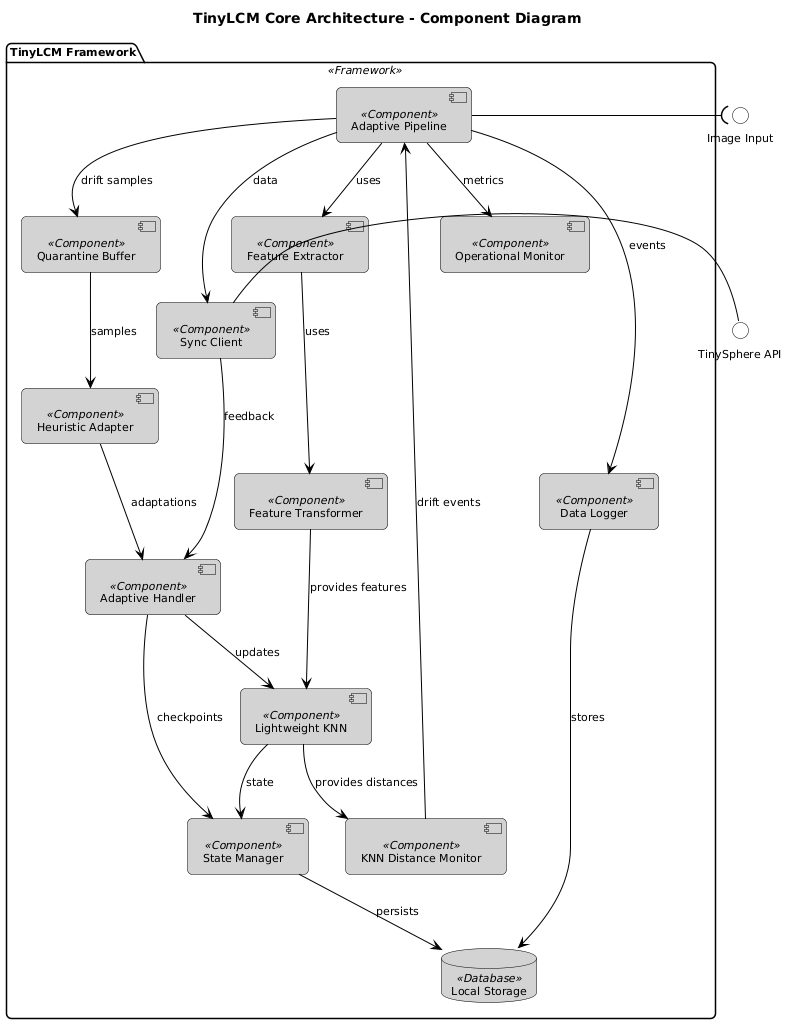
\includegraphics[width=0.65\textwidth]{figs/framework/tinylcm-component-dia.png}
    \caption[Component Diagram of the TinyLCM Core Library]{Component Diagram of the \gls{tinylcm} Core Library, illustrating its main modules and their interdependencies.}
    \label{fig:tinylcm_component_diagram}
\end{figure}

\begin{itemize}
    \item \textit{Pipeline Orchestration (\texttt{AdaptivePipeline}):} This central component, extending a base \texttt{InferencePipeline}, orchestrates the entire on-device workflow. It manages the sequence of operations from data ingestion and feature processing to classification, continuous monitoring, drift detection, and the initiation of adaptation routines.
    \item \textit{Feature Processing Subsystem:} Responsible for transforming raw input data (e.g., images) into a numerical representation suitable for the \gls{ml} model. This subsystem includes the \textit{\texttt{TFLiteFeatureExtractor}}, which utilizes a pre-trained, optimized \gls{tfl} model to extract high-dimensional feature vectors, and the \textit{\texttt{StandardScalerPCATransformer}}, which applies statistical normalization (z-score standardization) and dimensionality reduction to these vectors. The latter step is crucial for reducing computational load and enhancing the performance of subsequent components \cite{disabatoTinyMachineLearning2024}.
    \item \textit{Classification (\texttt{LightweightKNN}):} Performs the primary inference task using an optimized \gls{knn} algorithm, designed for a low memory footprint and computational efficiency. It stores a bounded number of reference samples and provides prediction confidence scores. Its internal state (neighbor distances) is also leveraged by the drift detection mechanism.
    \item \textit{Drift Detection Subsystem (\texttt{KNNDistanceMonitor}):} Implements algorithms for autonomous, on-device drift detection without requiring ground truth labels. The \texttt{KNNDistanceMonitor} tracks the average distance to ``k-nearest neighbors'' in the feature space and employs the Page-Hinkley statistical test to detect significant distributional shifts.
    \item \textit{Adaptation System:} Triggered by the \texttt{AdaptivePipeline} upon drift detection, this system manages the on-device model adaptation process. Key components include the \texttt{QuarantineBuffer}, which temporarily stores input samples flagged by drift detectors or exhibiting anomalous characteristics for analysis or potential use in adaptation; the \texttt{HeuristicAdapter}, which analyzes samples from the \texttt{QuarantineBuffer} and applies heuristic rules (e.g., feature space clustering) to generate pseudo-labels; and the \textit{\texttt{AdaptiveHandler}}, which manages the application of these pseudo-labeled samples to update the on-device model in a controlled manner.
    \item \textit{State Management and Persistence:} Ensures system robustness and recoverability. The \texttt{StateManager} handles versioning and persistent storage (e.g., as JSONL files on an SD card) of critical states, including the classifier's model and reference statistics for drift detectors, enabling rollbacks. The \texttt{DataLogger} records operational logs, inference results, drift events, and adaptation attempts. An \texttt{AdaptationTracker} logs details and outcomes of adaptation events.
    \item \textit{Operational Monitoring (\texttt{OperationalMonitor}):} Continuously tracks on-device performance metrics such as inference latency, CPU utilization, memory usage, and component operational status. This data is valuable for local diagnostics and can be synchronized with TinySphere.
    \item \textit{Synchronization Client (\texttt{SyncClient}):} Manages optional, opportunistic communication with the TinySphere server. This includes packaging data (logs, metrics, drift events, quarantined samples), handling intermittent network connectivity, and processing feedback or updates from the server.
\end{itemize}

This modular and configurable component-based architecture allows \gls{tinylcm} to be adapted to a wide range of applications and hardware platforms, such as \glspl{sbc}.

\subsection{Lightweight KNN Classifier}
\label{ssec:LightweightKNN}

A pivotal component within \gls{tinylcm}, enabling both classification and serving as a basis for drift detection, is the \texttt{LightweightKNN} classifier. This choice is informed by analyses in Chapter~\ref{chp:Research_Results} (specifically Section~\ref{sec:RQ2_Results_Frameworks}) and findings in the literature \cite{disabatoTinyMachineLearning2024} that highlight the suitability of KNN-based approaches for resource-constrained environments due to their potential for low inference cost and incremental updatability.

The \texttt{LightweightKNN} implementation incorporates several critical design decisions and optimizations:
\begin{itemize}
    \item \textit{Bounded Sample Storage for Memory Management:} To prevent uncontrolled memory consumption during long-term operation, the classifier stores its reference feature vectors, corresponding labels, and their arrival timestamps in Python \texttt{collections.deque} objects with a configurable \texttt{maxlen} attribute (\texttt{max\_samples}). This ensures the memory footprint for reference data remains strictly bounded, as oldest samples are automatically evicted when buffer capacity is exceeded—a crucial tactic for RAM optimization.
    \item \textit{Flexible and Efficient Distance Computation:} The classifier supports multiple distance metrics (e.g., Euclidean, Manhattan, Cosine) via a \texttt{DistanceCalculator} utility class. While optimized NumPy calculations are preferred for speed if available and the \texttt{use\_numpy} flag is set, pure Python implementations serve as fallbacks, ensuring broader compatibility.
    \item \textit{Confidence Score Calculation:} For each prediction, a confidence score is calculated. While various schemes exist, such as complex distance-weighting, a common alternative chosen here for stability in drift detection contexts is the simple proportion of votes from the \gls{knn} belonging to the predicted class. This score can be used by downstream components.
    \item \textit{Deterministic Tie-Breaking in Predictions:} In cases where multiple classes receive an equal number of votes among the \gls{knn}, a deterministic tie-breaking mechanism is employed, using sample timestamps. This ensures reproducible prediction outcomes.
    \item \textit{Provision of Neighbor Information for Drift Detection:} A key function is that \texttt{LightweightKNN} makes the distances to, and identities of, the\gls{knn} accessible after each prediction. This internal state is directly consumed by the \texttt{KNNDistanceMonitor}, avoiding redundant distance calculations by the monitor.
\end{itemize}

The core simplified logic, emphasizing efficient distance computation, neighbor selection, and voting, is illustrated in Listing~\ref{lst:lightweightknn_predict}.

\begin{lstlisting}[captionpos=b, language=Python, commentstyle=\color{blue}\itshape, caption={Example logic of the LightweightKNN Class}, label=lst:lightweightknn_predict]
class LightweightKNN:    
    def __init__(self, k=5, max_samples=1000, distance_metric='euclidean'):
        self.samples = deque(maxlen=max_samples)
        self.labels = deque(maxlen=max_samples)
        self.timestamps = deque(maxlen=max_samples)
        self.k = k
        self.distance_metric = distance_metric
        
    def predict(self, features):
        """Predict with neighbor tracking for drift detection."""
        if len(self.samples) < self.k:
            return None, 0.0
            
        # Compute distances efficiently
        distances = self._compute_distances(features)
        
        # Get k nearest neighbors
        k_nearest = sorted(enumerate(distances), key=lambda x: x[1])[:self.k]
        indices = [idx for idx, _ in k_nearest]
        
        # Vote counting with tie-breaking
        label_votes = defaultdict(lambda: {'count': 0, 'min_timestamp': float('inf')})
        for idx in indices:
            label = self.labels[idx]
            label_votes[label]['count'] += 1
            label_votes[label]['min_timestamp'] = min(
                label_votes[label]['min_timestamp'], 
                self.timestamps[idx]
            )
        
        # Determine winner with timestamp tie-breaking
        winner = max(label_votes.items(), 
                    key=lambda x: (x[1]['count'], -x[1]['min_timestamp']))[0]
        
        # Calculate confidence
        confidence = label_votes[winner]['count'] / self.k
        
        # Store neighbor info for drift detection
        self._store_neighbor_info(indices, distances, k_nearest)
        
        return winner, confidence
\end{lstlisting}

\subsection{Autonomous Drift Detection and Adaptation Mechanisms}
\label{ssec:tinylcm_drift_adaptation}

A defining characteristic of \gls{tinylcm}'s on-device \gls{lcm} is its capacity for autonomous concept drift detection and subsequent model adaptation. This approach directly addresses a critical challenge of frequent unavailability of real-time ground truth labels. \gls{tinylcm}'s autonomy is realized through an integrated system of statistical feature-space monitoring and heuristic-driven learning mechanisms, orchestrated within the \texttt{AdaptivePipeline}.

\paragraph{KNN-Distance Monitoring with Page-Hinkley Test}
Traditional drift detection methods often depend on true labels to monitor model performance \cite{disabatoTinyMachineLearning2024, pavanTyBoxAutomaticDesign2024}. \gls{tinylcm} therefore employs unsupervised drift detection by monitoring the statistical properties of input data within a learned feature space. The premise is that concept drift—a change in $P(X)$ or $P(Y|X)$ \cite{gamaSurveyConceptDrift2014}—often manifests as a discernible shift in how new data relates to an established reference distribution.

The process begins with the \texttt{TFLiteFeatureExtractor} transforming raw input data into a high-dimensional feature space. These features are then processed by the \texttt{StandardScalerPCATransformer}, which applies L2-normalization (Equation~\ref{eq:l2_norm_chap5_v2}), z-score standardization (Equation~\ref{eq:z_score_chap5_v2}), and PCA (Equation~\ref{eq:pca_transform_chap5_v2}). This pipeline, for instance, can reduce feature vectors from 1280 to 256 dimensions, normalizing feature scales and mitigating the curse of dimensionality, thereby enhancing the robustness of distance-based metrics used subsequently \cite{jolliffePrincipalComponentAnalysis2016}. The selection of these techniques aligns with common practices in \gls{tinyml} for preprocessing data efficiently, as discussed in Chapter~\ref{chp:Research_Results} concerning data-centric architectures.

Within this transformed, lower-dimensional feature space, the \texttt{LightweightKNN} classifier (Section~\ref{ssec:LightweightKNN}) provides not only predictions but also the Euclidean distances to the $k$-nearest neighbors for each query point (Equation~\ref{eq:euclidean_distance_chap5_v2}). The \texttt{KNNDistanceMonitor} component utilizes the average of these $k$ distances, denoted $x_t$ (Equation~\ref{eq:drift_signal_chap5_v2}), as a sensitive proxy metric. A statistically significant, sustained increase in $x_t$ suggests incoming data points are becoming dissimilar to the reference data, indicating a potential distribution shift.

To formally detect such changes, the \texttt{KNNDistanceMonitor} employs the Page-Hinkley test \cite{pageContinuousInspectionSchemes1954}, a sequential analysis technique well-suited for detecting persistent changes in a signal's mean. Given the time series of average \gls{knn} distances $x_t$, a reference mean distance $\mu_0$ (established during an initial warm-up phase), and a tolerance parameter $\delta > 0$, the Page-Hinkley test statistics are updated incrementally (Equations~\ref{eq:ph_mt_chap5_v2} through \ref{eq:ph_statistic_chap5_v2}).

Let \(\mathbf{f}_{\mathrm{raw}}\in\mathbb{R}^D\) denote the raw feature vector. L\(^2\)-normalization yields:
\begin{flalign}
  && \mathbf{f}_{\mathrm{norm}}
   = \frac{\mathbf{f}_{\mathrm{raw}}}{\|\mathbf{f}_{\mathrm{raw}}\|_2},
  \qquad
  \|\mathbf{f}_{\mathrm{raw}}\|_2
   = \sqrt{\sum_{i=1}^D f_{\mathrm{raw},i}^2}. &&
   \label{eq:l2_norm_chap5_v2}
\end{flalign}
Standardization and PCA transformation follow:
\begin{flalign}
  && \mathbf{z}
   = \frac{\mathbf{f}_{\mathrm{norm}} - \boldsymbol{\mu}_{\mathrm{norm}}}
         {\boldsymbol{\sigma}_{\mathrm{norm}}}, &&
   \label{eq:z_score_chap5_v2}\\
  && \mathbf{y}
   = \mathbf{z}\,W,
  \qquad
  \mathbf{y}\in\mathbb{R}^K. &&
   \label{eq:pca_transform_chap5_v2}
\end{flalign}
The Euclidean distance to a neighbor $\mathbf{r}_j$ for a point $\mathbf{y}_t$ is:
\begin{flalign}
  && d(\mathbf{y}_t,\mathbf{r}_j)
   = \sqrt{\sum_{i=1}^K \bigl(y_{t,i} - r_{j,i}\bigr)^2}, &&
   \label{eq:euclidean_distance_chap5_v2}
\end{flalign}
leading to the average KNN distance (drift signal):
\begin{flalign}
  && x_t = \frac{1}{k}\sum_{j=1}^k d(\mathbf{y}_t,\mathbf{r}_j). &&
   \label{eq:drift_signal_chap5_v2}
\end{flalign}
The Page-Hinkley test statistics are then:
\begin{flalign}
  && m_t = m_{t-1} + \bigl(x_t - \mu_0 - \delta\bigr), \quad \text{with } m_0 = 0, &&
   \label{eq:ph_mt_chap5_v2}\\
  && M_t = \min\bigl(M_{t-1},\,m_t\bigr), \quad \text{with } M_0 = 0, &&
   \label{eq:ph_Mt_chap5_v2}\\
  && PH_t = m_t - M_t. &&
   \label{eq:ph_statistic_chap5_v2}
\end{flalign}

A drift is flagged if $PH_t$ exceeds a predefined detection threshold $\lambda$. The operational flow of the \texttt{KNNDistanceMonitor}, including hysteresis and cooldown periods to prevent alarm flooding—a practical consideration for stable autonomous systems is detailed in Algorithm~\ref{alg:knn_distance_monitor_update}.

\begin{algorithm}[htbp]
  \caption{Update procedure for the \texttt{KNNDistanceMonitor}}
  \label{alg:knn_distance_monitor_update}
  \begin{algorithmic}[1]
    \Require Current average KNN distance $x_t$; Reference mean $\mu_0$; Tolerance $\delta$; Detection threshold $\lambda$; Exit threshold $\lambda_{\mathrm{exit}}$; Current Page-Hinkley sums $m_{t-1}, M_{t-1}$; Warm-up data buffer $W$; Warm-up phase flag $is\_warmup$; Reference initialized flag $ref\_initialized$; In drift state flag $in\_drift\_state$.
    \If{$is\_warmup$}
      \State Add $x_t$ to $W$.
      \State \Return \textbf{no drift}
    \ElsIf{not $ref\_initialized$}
      \State $\mu_0 \gets \mathrm{mean}(W)$; $\sigma_0 \gets \mathrm{std}(W)$ \Comment{Initialize reference from warm-up data}
      \State $m_t \gets 0$; $M_t \gets 0$ \Comment{Initialize Page-Hinkley statistics}
      \State $ref\_initialized \gets \textbf{true}$
      \State \Return \textbf{no drift}
    \Else
      \State $m_t \gets m_{t-1} + (x_t - \mu_0 - \delta)$
      \State $M_t \gets \min(M_{t-1}, m_t)$
      \State $PH_t \gets m_t - M_t$
      \If{not $in\_drift\_state$ and $PH_t > \lambda$}
        \State $in\_drift\_state \gets \textbf{true}$
        \State \Return \textbf{drift detected}
      \ElsIf{$in\_drift\_state$ and $PH_t \le \lambda_{\mathrm{exit}}$}
        \State $in\_drift\_state \gets \textbf{false}$
        \State $m_t \gets 0$; $M_t \gets 0$ \Comment{Reset Page-Hinkley statistics}
        \State \Return \textbf{drift ended}
      \Else
        \State \Return \textbf{no drift (or still in drift)}
      \EndIf
    \EndIf
  \end{algorithmic}
\end{algorithm}
\FloatBarrier

\paragraph{Heuristic Pseudo-Labeling and Quarantine}
Upon significant drift detection, \gls{tinylcm}'s \texttt{AdaptivePipeline} initiates an on-device adaptation process. This process, depicted in Figure~\ref{fig:heuristic_adaptation_sequence_diagram}, is engineered for immediate yet cautious response. It leverages a heuristic-based pseudo-labeling strategy to update the on-device model, aiming for adaptation without requiring immediate external ground truth. This contrasts with more resource-intensive on-device retraining approaches discussed in Chapter~\ref{chp:Research_Results} (e.g., full backpropagation), and is chosen for its balance of responsiveness and computational frugality, suitable for \glspl{mcu}.

\begin{figure}[htbp]
    \centering
    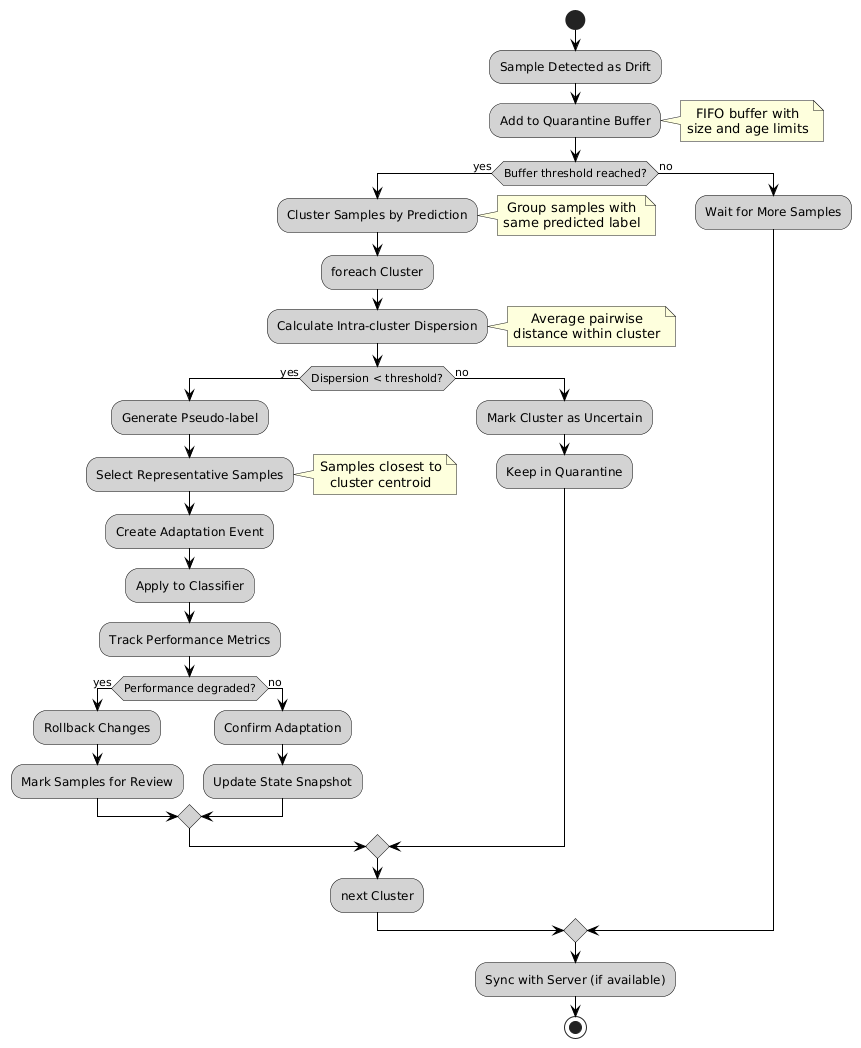
\includegraphics[width=0.75\textwidth]{figs/framework/heuristic-adaptation-activity.png}
    \caption[Activity Diagram of the Heuristic Adaptation Process]{Activity Diagram detailing the heuristic adaptation logic}
    \label{fig:heuristic_adaptation_sequence_diagram}
\end{figure}
\FloatBarrier

The on-device adaptation cycle involves the following stages:
\begin{itemize}
    \item \textit{Quarantine Buffer Management:} Input samples triggering a drift alert, or subsequent samples with similar anomalous characteristics, are moved to the \texttt{QuarantineBuffer}. This FIFO buffer, with configurable size and sample age limits, collects a small, manageable set of these ``unusual'' samples for focused analysis.
    \item \textit{Heuristic Pseudo-Labeling by \texttt{HeuristicAdapter}:} The \texttt{HeuristicAdapter} analyzes feature vectors of samples in the \texttt{QuarantineBuffer}. A core heuristic involves clustering these quarantined samples within their PCA-transformed feature space. Samples might be grouped based on their original (potentially incorrect) \texttt{LightweightKNN} prediction or via unsupervised clustering if no prior prediction is reliable. If a sufficiently distinct and cohesive cluster of new, anomalous samples forms, it may be inferred that these samples represent a novel or significantly shifted concept. A pseudo-label is then assigned (e.g., based on the predominant original label if cohesive, or a new ``unknown'' label if distinct). Confidence in such pseudo-labels can be derived from metrics like intra-cluster dispersion, cluster size, and separation from existing class centroids.
    \item \textit{Cautious Model Update via \texttt{AdaptiveHandler}:} Adaptation events, containing representative samples from a confident pseudo-labeled cluster, are passed to the \texttt{AdaptiveHandler}. This component cautiously updates the \texttt{LightweightKNN} classifier by adding these pseudo-labeled samples to its reference set.
    \item \textit{Post-Adaptation Performance Monitoring and Rollback:} Following adaptation, the \texttt{AdaptiveHandler} and \texttt{OperationalMonitor} continue to track performance. If metrics indicate performance degradation, a rollback to the previously saved state can be automatically triggered via the \texttt{StateManager}. Samples causing detrimental adaptation may be flagged for mandatory server review.
    \item \textit{Opportunistic External Validation:} Pseudo-labeled samples, their generation context, and adaptation outcomes are packaged by the \texttt{SyncClient}. This package is queued for optional, asynchronous transmission to TinySphere when connectivity permits. TinySphere can then employ more sophisticated validation (e.g., human-in-the-loop analysis) to confirm/refute pseudo-labels. This validated feedback can subsequently refine \gls{tinylcm} models during future synchronizations, aligning with the concept of the Active/Passive handlers used in \cite{disabatoIncrementalOnDeviceTiny2020,disabatoTinyMachineLearning2024}.
\end{itemize}

This adaptive loop—combining autonomous detection, heuristic-based learning, robust state management, and optional external validation—allows \gls{tinylcm} to dynamically evolve its understanding of the operational environment and maintain performance despite changing data distributions, a key aspect of robust \gls{lcm} practices discussed as emerging in Chapter~\ref{chp:Research_Results}.

\begin{MyBox}{\textbf{Implementation Status of On-Device Heuristic Adaptation}}
    It is important to note that the on-device heuristic pseudo-labeling and adaptation logic described represents a conceptual and architectural design developed for this thesis. While the overall workflow and component interactions (e.g., with the \texttt{QuarantineBuffer} and \texttt{AdaptiveHandler}) are defined, the specific algorithms for heuristic pseudo-label generation and their efficient, resource-aware implementation have not yet been fully realized and tested.
\end{MyBox}

\paragraph{State Management for Resilience}
To ensure operational resilience, particularly when autonomous adaptations may not consistently yield improvements, \gls{tinylcm} incorporates a robust \texttt{AdaptiveStateManager}. This component is crucial because on-device adaptations, while aiming to maintain performance in dynamic environments, risk issues such as catastrophic forgetting or incorrect learning from noisy data, especially when ground truth is absent \cite{renOndeviceOnlineLearning2024, pavanTyBoxAutomaticDesign2024}. The \texttt{AdaptiveStateManager} mitigates these risks by versioning the state of critical components, primarily the \texttt{LightweightKNN} classifier's reference set (features, labels, and timestamps), enabling rollbacks to known-good configurations.

The core mechanism involves saving the classifier's current state \textit{before} any on-device adaptation is applied. This snapshot, including the KNN's reference samples, a version identifier, and a timestamp, is serialized to non-volatile storage. A key consideration for resource-constrained devices is the performance impact of this save operation. Therefore, as illustrated in Listing~\ref{lst:statemanager}, this operation is handled asynchronously using a dedicated worker thread and task queue. This non-blocking approach prevents the main inference pipeline from stalling.

If subsequent evaluation—either through \gls{tinylcm}'s on-device monitoring of proxy metrics or via feedback from TinySphere (Section~\ref{sec:tinysphere_detailed_design})—indicates that an adaptation has degraded performance, a rollback is triggered. The \texttt{AdaptiveStateManager} then restores the \texttt{LightweightKNN} classifier to its previously saved, validated state. To manage limited storage resources effectively, the state manager also implements a policy for pruning old or superseded snapshots.

\begin{lstlisting}[captionpos=b, language=Python, commentstyle=\color{blue}\itshape, caption={\texttt{AdaptiveStateManager} Implementation Highlights}, label=lst:statemanager]
class AdaptiveStateManager:
    
    def __init__(self, storage_path: Path, max_snapshots: int = 10):
        self.storage_path = storage_path
        self.max_snapshots = max_snapshots
        self.worker_thread = Thread(target=self._worker, daemon=True)
        self.task_queue = Queue()
        self.worker_thread.start()
        
    def create_snapshot(self, pipeline_state: dict, metadata: dict):
        """Create state snapshot asynchronously."""
        snapshot = {
            'timestamp': datetime.now().isoformat(),
            'state_version': 2,
            'pipeline_state': pipeline_state,
            'metadata': metadata
        }
        
        self.task_queue.put(('save', snapshot))
        
    def rollback_to_snapshot(self, snapshot_id: str) -> dict:
        """Restore system state from snapshot."""
        snapshot_path = self.storage_path / f"{snapshot_id}.json"
        with open(snapshot_path, 'r') as f:
            snapshot = json.load(f)
            
        if snapshot['state_version'] != 2:
            raise ValueError(f"Incompatible state version: {snapshot['state_version']}")
            
        return snapshot['pipeline_state']
\end{lstlisting}

\section{TinySphere: A TinyML-Centric Server Platform for Enhanced MLOps}
\label{sec:tinysphere_detailed_design}

While \gls{tinylcm} provides the foundational layer for on-device autonomy, the TinySphere platform serves as its optional, yet deeply integrated, server-side counterpart. TinySphere is specifically architected to extend traditional \gls{mlops} capabilities, such as those offered by MLflow, with functionalities tailored to the unique operational lifecycle and data characteristics of fleets of adaptive \gls{tinyml} devices. It is not merely a generic \gls{mlops} backend but a purposeful extension designed to seamlessly integrate with \gls{tinylcm}-enabled devices, understand their autonomously generated data, and provide a centralized hub for validation, monitoring, advanced analytics, and fleet management. This section outlines the rationale for TinySphere, details its architectural design, and highlights its key contributions to the comprehensive TinyMLOps ecosystem.

\subsection{Rationale and Objectives for a TinyML-Centric MLOps Platform}
\label{ssec:tinysphere_rationale}

The imperative for developing TinySphere stems from the observation, articulated in Section~\ref{ssec:framework_revisiting_gaps}, that existing \gls{mlops} platforms often fall short when addressing the specific needs of managing autonomous, adaptive fleets of TinyML devices operating at the extreme edge. While powerful tools like Edge Impulse excel in the initial model development and deployment phases \cite{banburyEdgeImpulseMLOps2023}, and platforms such as MLflow provide robust components for generic experiment tracking and model versioning in conventional ML workflows \cite{condeEnhancedFIWAREBasedArchitecture2024}, a dedicated platform is required to effectively:
\begin{itemize}
    \item \textit{TinyML-Specific Data Streams:} Handle the unique data packages originating from \gls{tinylcm}-enabled devices, which include drift events detected via proxy metrics, heuristically generated pseudo-labels, on-device adaptation logs, and resource-constrained operational telemetry.
    \item \textit{Asynchronous Validation of On-Device Decisions:} Provide mechanisms for the external, potentially human-in-the-loop, validation of autonomous on-device adaptations. This is crucial for ensuring the long-term reliability and correctness of unsupervised learning processes occurring at the edge.
    \item \textit{Enable Centralized Monitoring and Comparative Analytics:} Aggregate operational data from a distributed fleet of resource-constrained devices to provide a centralized overview of system health, model performance across diverse environments, and emergent drift patterns.
    \item \textit{Tailored Model Management and Deployment Strategies:} Support model management and deployment workflows that explicitly account for the severe constraints (e.g., limited bandwidth, intermittent connectivity, heterogeneous hardware) and unique update mechanisms (e.g., \gls{tinylcm}'s model pull strategy) of TinyML targets.
    \item \textit{Edge Autonomy with Centralized Oversight:} Create a unified \gls{lcm} framework that respects and leverages on-device autonomy while providing the benefits of centralized MLOps for tasks where scale, computational power, or human expertise are indispensable.
\end{itemize}

\subsection{Architectural Design of TinySphere}
\label{ssec:tinysphere_architecture}

TinySphere is implemented as a modern, microservices-oriented web application. Its backend is built using FastAPI, chosen for its high performance, asynchronous capabilities, and automatic OpenAPI documentation generation, providing a robust and scalable RESTful API for communication with \gls{tinylcm} clients and the web dashboard. For data persistence, TinySphere employs a dual-storage strategy: (i) a PostgreSQL database is utilized for storing structured relational data, such as device metadata, drift event summaries, package information, and processed metrics; (ii) MinIO, an S3-compatible object storage solution, is used for managing larger binary artifacts, including uploaded device packages, images associated with drift events, full operational logs, and model files.

A cornerstone of TinySphere's design is its extension of, and integration with, MLflow. Rather than reinventing established MLOps components, TinySphere leverages MLflow for core functionalities like experiment tracking and model registry, while building specialized TinyML-centric services around it. The overall architecture, illustrated in Figure~\ref{fig:tinysphere_architecture_diagram}, delineates the API layer, service layer, data persistence layer, and its interaction with external systems and the edge devices.

\begin{figure}[htbp]
    \centering
    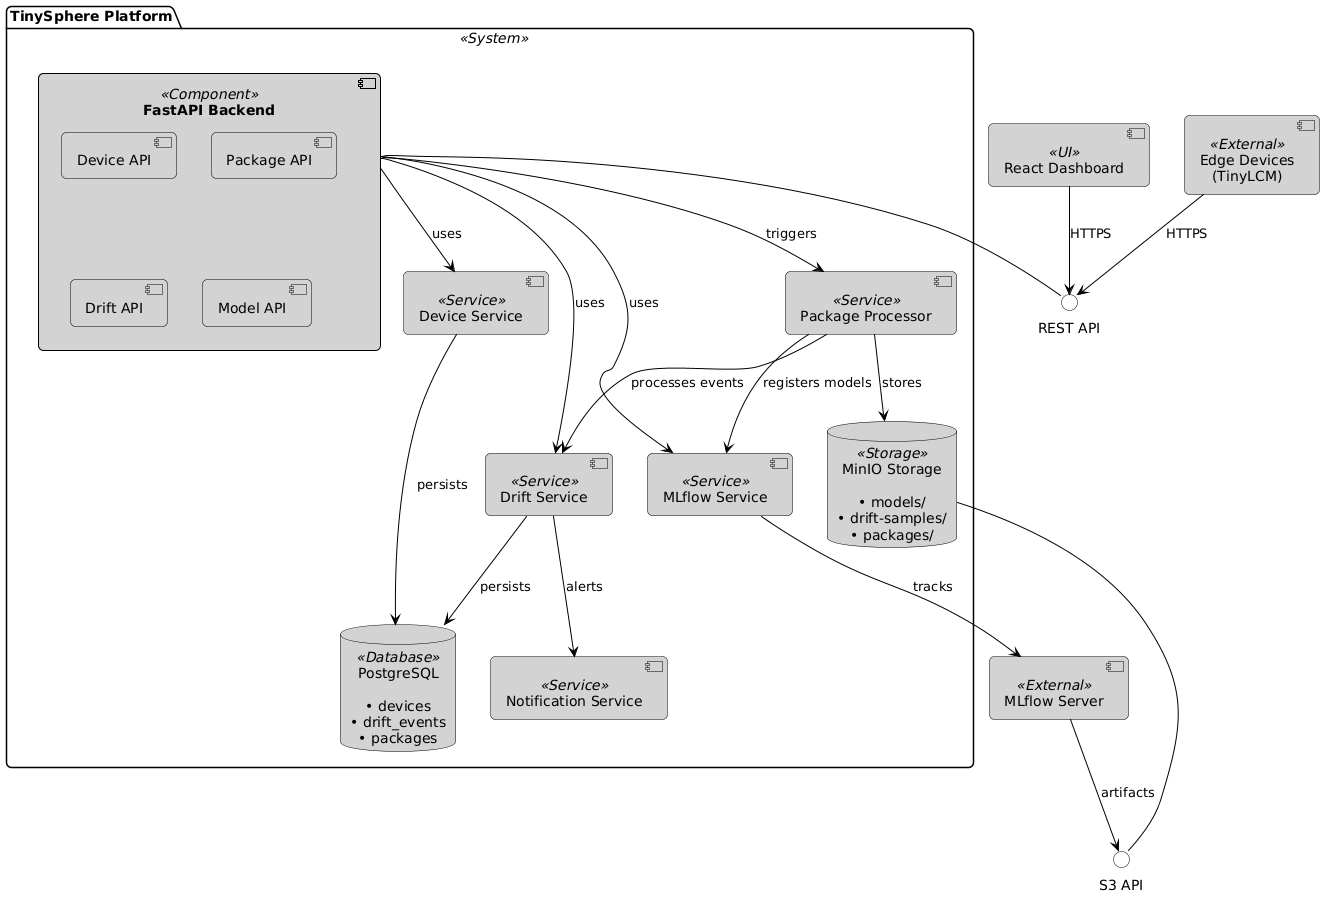
\includegraphics[width=0.95\textwidth]{figs/framework/tinysphere-architecture.png}
    \caption[Architectural Design of the TinySphere Server Platform]{Architectural Component Diagram of the TinySphere Server Platform}
    \label{fig:tinysphere_architecture_diagram}
\end{figure}

Key architectural components within TinySphere include:
\begin{itemize}
    \item \textit{API Layer}: Provides RESTful endpoints for all external interactions. This includes distinct routers for device management (`Device API`), package uploads and processing (`Package API`), drift event querying and validation (`Drift API`), and model management interactions (`Model API`).
    \item \textit{MLflow Service}: Orchestrates interactions with the MLflow tracking server and model registry, for example, when processing model-related information from device packages or logging server-side (re)training experiments.
    \item \textit{Drift Service}: Manages the lifecycle of drift events reported by devices, from initial ingestion and storage of associated samples and metadata to facilitating their validation workflow and tracking resolution status.
    \item \textit{Device Service}: Handles device registration, maintains a registry of active devices, tracks their status (e.g., connectivity, platform details, \gls{tinylcm} version), and manages associated metadata such as geolocation.
    \item \textit{Package Processor}: An extensible, multi-stage pipeline responsible for receiving, extracting, and processing the diverse data packages uploaded by \gls{tinylcm} devices. It detects package types (e.g., model, metrics, drift, operational logs) and routes their contents to appropriate transformers and services for storage and analysis.
    \item \textit{PostgreSQL Database}: Stores structured, relational data, including device registry, drift event metadata, package tracking information, and aggregated metrics for dashboarding.
    \item \textit{MinIO Object Storage}: Provides scalable storage for binary artifacts, such as original uploaded packages, extracted drift samples (images, features), model files, and extensive operational logs.
    \item \textit{Frontend (Web Dashboard)}: A React-based web application, providing an interactive interface for ML engineers and data scientists to monitor the device fleet, manage devices, review and validate drift events, inspect operational data, and interact with the model registry. An iullustrative mockup of this interface is shown in Figure~\ref{fig:uitinysphere}.
\end{itemize}

\subsection{Key MLOps Capabilities Provided by TinySphere}
\label{ssec:tinysphere_capabilities}

TinySphere is designed to deliver a suite of MLOps capabilities, extending the autonomous operations of \gls{tinylcm}-enabled devices:

\begin{itemize}
    \item \textit{Package Processing and Data Transformation}: TinySphere's `PackageProcessor` implements a sophisticated pipeline that can automatically detect the type of incoming data packages from \gls{tinylcm} devices and route them to a series of appropriate data transformers. For example, a `ModelTransformer` might register a new on-device model version with MLflow and store its artifact in MinIO; a `MetricsTransformer` could extract performance data and log it as an MLflow experiment/run; a `DriftTransformer` processes drift event details and stores associated samples for review; and an `OperationalLogsTransformer` parses raw log entries for aggregation and analysis. This automated pipeline, illustrated in Figure~\ref{fig:package_processing_pipeline}, ensures that data from the edge is efficiently ingested, processed, and made available for various MLOps workflows.

    \begin{figure}[htbp]
        \centering
        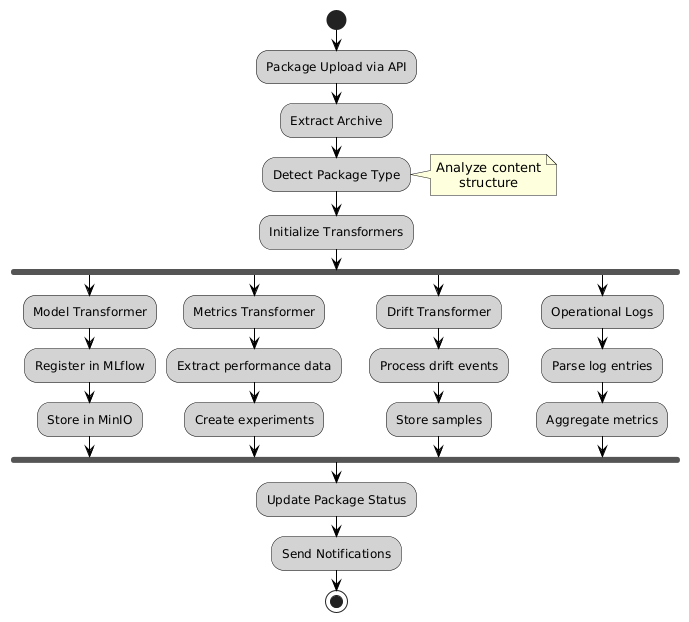
\includegraphics[width=0.7\textwidth]{figs/framework/package-processing-pipeline.png}
        \caption[Package Processing Pipeline in TinySphere]{Activity Diagram of the TinySphere Package Processing Pipeline}
        \label{fig:package_processing_pipeline}
    \end{figure}

    \item \textit{Drift Management}: TinySphere provides a dedicated system for managing and validating drift events. It supports various drift types (confidence-based, distribution-based, KNN-distance based). Reported drift samples are stored in MinIO, allowing human experts to review them via the TinySphere dashboard (``Drift Hub''). A structured validation workflow, depicted in Figure~\ref{fig:drift_validation_workflow}, enables experts to provide ground truth labels or confirm/reject on-device heuristic adaptations. This validated feedback, can then be synchronized back to the edge devices, facilitating a closed-loop learning process that refines on-device models with high-quality supervisory signals.

    \begin{figure}[htbp]
        \centering
        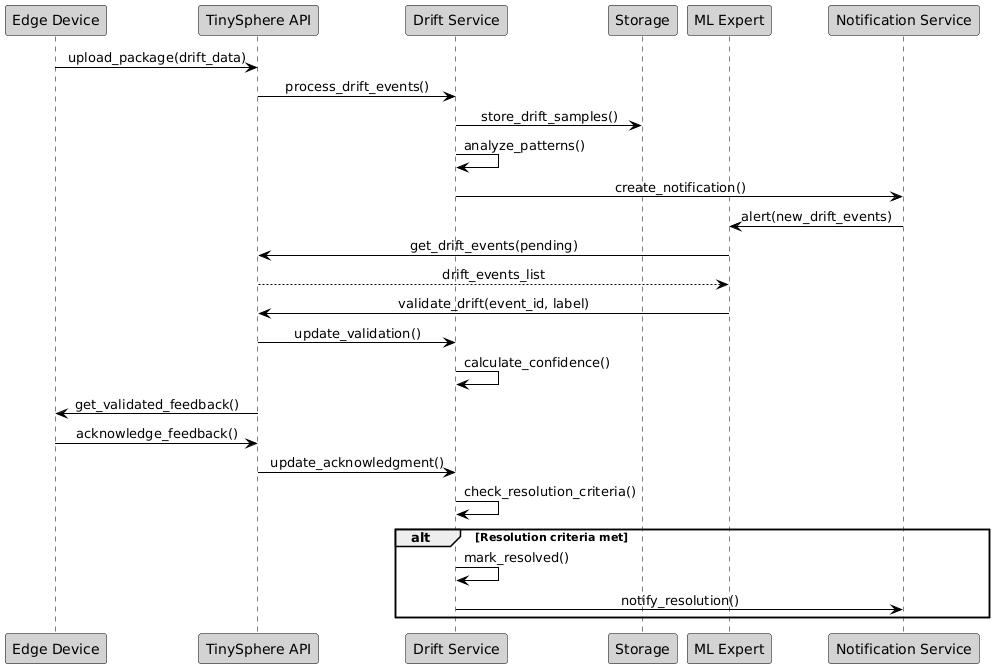
\includegraphics[width=0.9\textwidth]{figs/framework/drift-validation-workflow.png}
        \caption[Drift Validation Workflow in TinySphere]{Sequence Diagram illustrating the Drift Validation Workflow in TinySphere}
        \label{fig:drift_validation_workflow}
    \end{figure}

    \item \textit{Device Fleet Management}: The ``DeviceService'' within TinySphere maintains a registry of all connected \gls{tinylcm} devices, tracking their operational status, platform details (OS, \gls{tinylcm} version), connectivity (e.g., ``online'', ``offline'' based on last seen time), and, if provided by the device, geolocation data. This enables fleet-wide monitoring and allows for the correlation of model performance or drift occurrences with specific geographical regions or environmental contexts, visualized on the dashboard.

    \item \textit{Model Registry}: TinySphere seamlessly integrates with an MLflow server for its model registry capabilities. Models trained or fine-tuned based on fleet data, or even new base models intended for deployment, can be registered in MLflow. TinySphere extends this by associating TinyML-specific metadata with these models, such as their quantized size, target platform suitability, typical inference time on reference edge hardware, and configurations for associated feature extractors or drift detectors.
    \item \textit{Operational Monitoring}: By aggregating metrics and logs from \gls{tinylcm} devices, TinySphere provides a centralized dashboard for monitoring overall system health of deployed models.
\end{itemize}
These capabilities collectively position TinySphere as a specialized MLOps control plane, designed to augment the autonomy of \gls{tinylcm}-powered edge devices with robust, scalable, and insightful server-side operational management. Example mockups of the TinySphere user interface are provided in Figure~\ref{fig:uitinysphere}.

\begin{figure}[htbp]
    \centering
    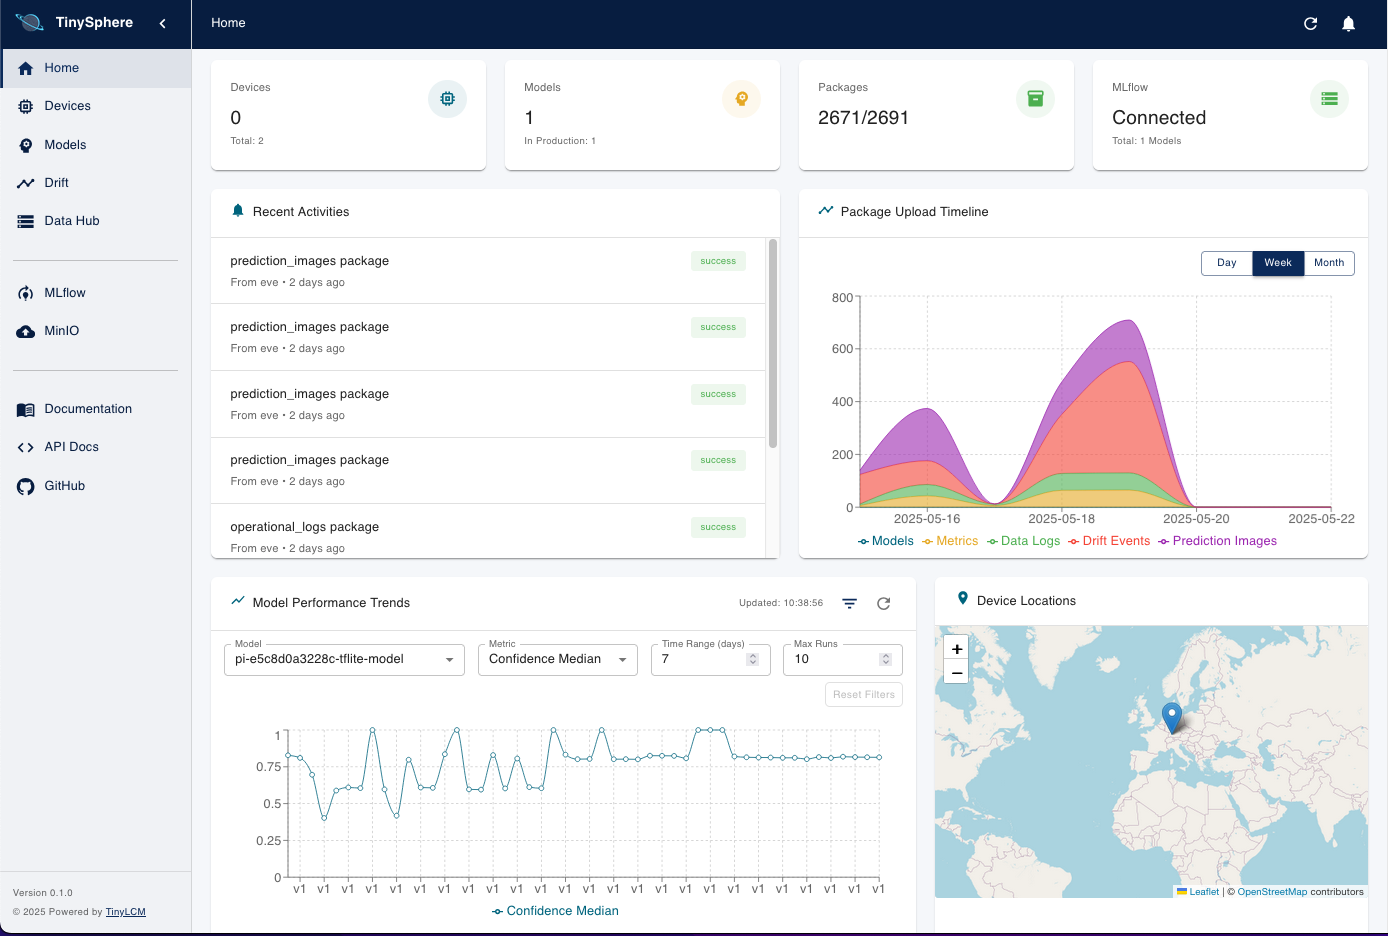
\includegraphics[width=0.975\textwidth]{figs/framework/ui-tinyssphere.png}
    \caption[User Interface of TinySphere]{User Interface of TinySphere, illustrating the dashboard for monitoring device status and drift events.}
    \label{fig:uitinysphere}
\end{figure}

\begin{MyBox}{\textbf{Note on TinySphere's Interaction with Conceptual Heuristic Adaptation}}
    Further to the implementation status of the on-device heuristic adaptation logic within \gls{tinylcm} (as noted in Section~\ref{sec:tinylcm_detailed_design}), it is important to reiterate that TinySphere's capabilities for processing, validating, and providing feedback on data originating from these specific adaptations are, by extension, also based on this conceptual foundation.
\end{MyBox}

\section{Exemplary Operational Workflow}
\label{ssec:ecosystem_workflow}

To illustrate the practical application and collaborative nature of the TinyMLOps ecosystem based on its current implementation state, this subsection outlines an exemplary end-to-end operational workflow. This workflow, particularly relevant for the Proof-of-Concept development (the Mars rover prototype), spans from initial local model development to continuous production operation involving on-device drift detection and server-assisted data analysis. The workflow is divided into three main phases, detailed below.

\textbf{Phase 1: Local Development and Initial Model Training}
The initial creation of the \gls{ml} model and essential \gls{tinylcm} artifacts occurs on a development machine, forming the foundation for edge deployment.
\begin{enumerate}
    \item \textit{Model Prototyping and Training:} An \gls{ml} engineer utilizes scripts (e.g., Python scripts leveraging TensorFlow/Keras) to perform transfer learning, typically using a pre-trained base model such as MobileNetV2, on a custom dataset relevant to the target application. This process culminates in a quantized \gls{tfl} model optimized for edge deployment, along with associated class labels.
    \item \textit{Feature Processor Generation:} Concurrently, the feature processing pipeline components, including the \texttt{StandardScaler} and \texttt{PCA} models, are fitted on features extracted from the training dataset. These fitted transformers are saved for on-device deployment.
    \item \textit{Initial State Generation for \gls{tinylcm}:} Specialized scripts are executed to create the initial state for the \texttt{LightweightKNN} classifier by populating it with a representative subset of the training data. Additionally, initial reference statistics for the \texttt{KNNDistanceMonitor} are computed based on the trained model and feature processor.
    \item \textit{Configuration File Preparation:} A scenario-specific JSON configuration file is meticulously prepared. This file defines paths to all necessary artifacts (model, scaler, PCA model, initial KNN state, labels) and specifies operational parameters for all \gls{tinylcm} components, including the feature extractor, classifier, drift detectors, and \texttt{SyncClient}.
    \item \textit{Version Control and Packaging:} All generated artifacts, configuration files, \gls{tinylcm} library code, and application-specific scripts are committed to a version control system (e.g., Git) and packaged for deployment.
\end{enumerate}

\textbf{Phase 2: Device Deployment and Autonomous Drift Detection}
Provisioning the target edge device and initiating \gls{tinylcm}'s autonomous operational loop—focused on inference and drift detection—constitute the second phase.
\begin{enumerate}
    \item \textit{Edge Device Preparation:} The target edge device is prepared with a suitable base operating system and necessary system dependencies.
    \item \textit{Installation and Setup:} The device executes an installation script fetched from the Git repository via `curl`. This script automates cloning the application repository, installing Python dependencies, copying specific scenario files to appropriate device locations, and establishing the directory structure for logs and state persistence.
    \item \textit{Initiation of Autonomous Execution:} The main application script is launched on the device. \gls{tinylcm}, configured via the JSON file, commences its autonomous operational loop: performing inference on input data; continuously monitoring for concept drift; and, if drift is detected, quarantining the relevant raw input samples and logging detailed event information using the \texttt{QuarantineBuffer} and \texttt{DataLogger}.
\end{enumerate}

\textbf{Phase 3: TinySphere Integration and Data Review for MLOps}
Synergistic interaction with TinySphere for enhanced \gls{mlops} capabilities, assuming opportunistic network connectivity, characterizes the third phase.
\begin{enumerate}
    \item \textit{Opportunistic Data Synchronization:} If configured to communicate with a TinySphere instance and network connectivity is available, \gls{tinylcm}'s \texttt{SyncClient} periodically (or upon specific triggers, such as a significant drift event) packages locally buffered data. This data includes operational logs, performance metrics, detailed drift event information, and the quarantined raw input samples associated with detected drift. These packages are then transmitted to the TinySphere API.
    \item \textit{Data Ingestion and Processing:} TinySphere's backend API receives these packages. Its \texttt{PackageProcessor} component validates, extracts, and routes the contained data to various specialized services and transformers. Operational logs and metrics are parsed for dashboard visualization. Drift event details and the associated raw samples are processed by a \texttt{DriftTransformer} and stored (e.g., images in MinIO, metadata in PostgreSQL), making them accessible via TinySphere's ``Data Hub'' (or ``Drift Hub'') interface for review by an \gls{ml} engineer.
    \item \textit{MLflow Integration for Experiment and Model Tracking:} An \texttt{MLflowService} within TinySphere can be used to log experiment runs related to model performance observed on devices. While on-device adaptations are not occurring, data from drift events or device telemetry can inform the tracking of deployed model behavior over time. New centrally trained model versions can be registered, with artifacts stored (e.g., in MinIO).
    \item \textit{Fleet Management, Monitoring, and Data Review:} \gls{ml} engineers and data scientists can utilize the TinySphere web interface (illustrative examples in Figure~\ref{fig:tinysphere_ui_examples}) to monitor the operational status of registered devices, view aggregated performance analytics, and, crucially, examine the quarantined raw samples and detailed drift events from across the fleet within the ``Data Hub''.
    \item \textit{Manual Data Labeling and Analysis:} Through the ``Data Hub'' UI, human operators can review the quarantined raw samples (e.g., images of unknown objects or inputs that triggered drift alerts) associated with drift events reported by devices. They can then manually assign ground truth labels to these samples. This manually labeled dataset becomes a valuable asset, stored by TinySphere.
    \item \textit{Model Improvement Cycle:} The manually labeled data, aggregated in TinySphere from various devices and drift events, serves as a curated dataset for model analysis and retraining. An \gls{ml} engineer can use this dataset to: (i) understand the nature of the drift, (ii) augment the training dataset, and (iii) trigger a central retraining cycle for the \texttt{LightweightKNN} or even the base feature extractor model. A new, improved model version, once validated centrally, can then be packaged (Phase 1) and subsequently deployed to the edge device(s) through an appropriate update mechanism (e.g., manual update, or a future automated deployment feature of TinySphere).
\end{enumerate}

This workflow, emphasizing on-device drift detection and server-assisted data collection for human-driven analysis and model evolution, demonstrates a pragmatic approach to managing TinyML applications and addresses operational complexities identified in Chapter~\ref{chp:Research_Results} within the bounds of the current implementation.

\begin{figure}[htbp]
    \centering

    \begin{subfigure}[b]{0.48\textwidth}
        \centering
        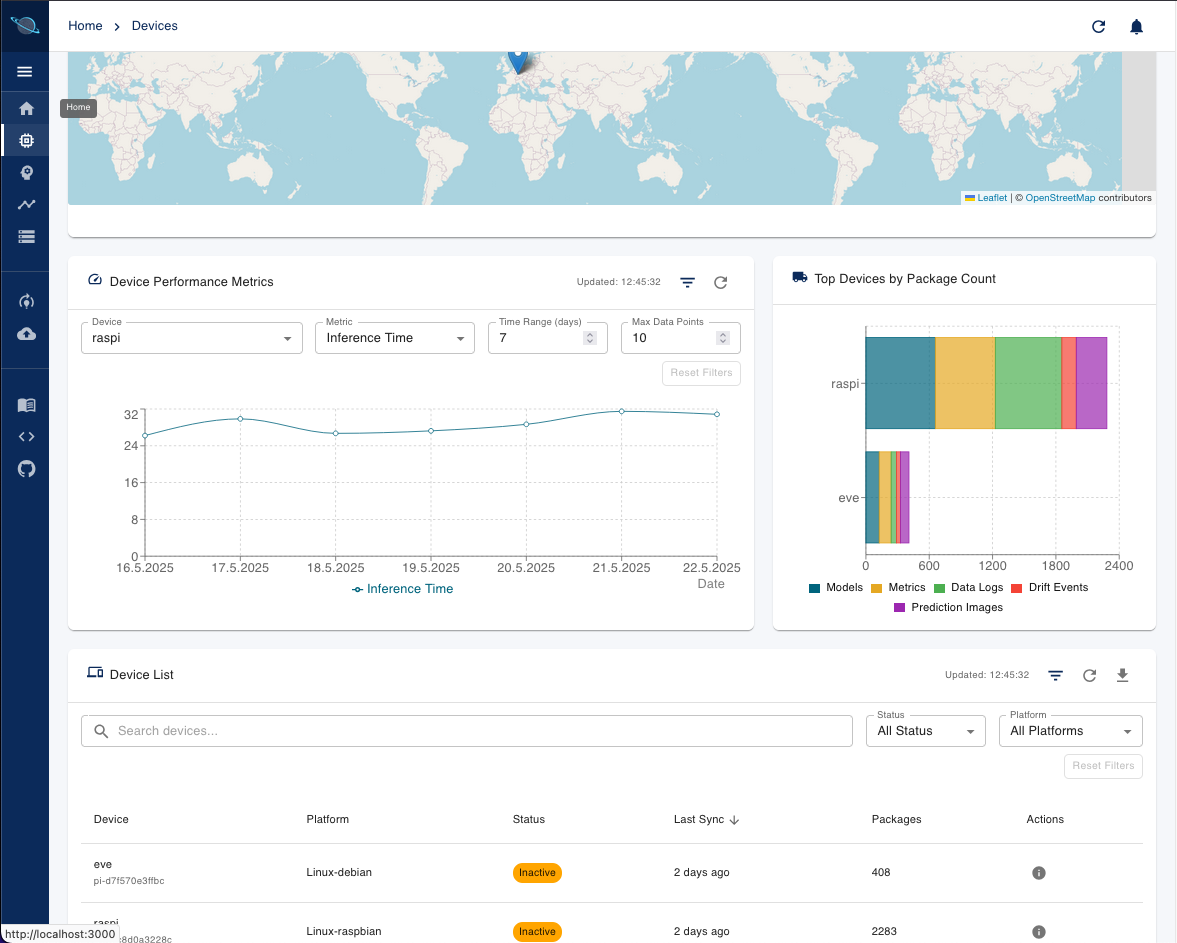
\includegraphics[width=\textwidth]{figs/framework/device-page.png}
        \caption{TinySphere device page providing an overview of the device fleet, including status, key statistics, and location data for individual devices.}
        \label{fig:ui_device_page}
    \end{subfigure}
    \hfill
    \begin{subfigure}[b]{0.48\textwidth}
        \centering
        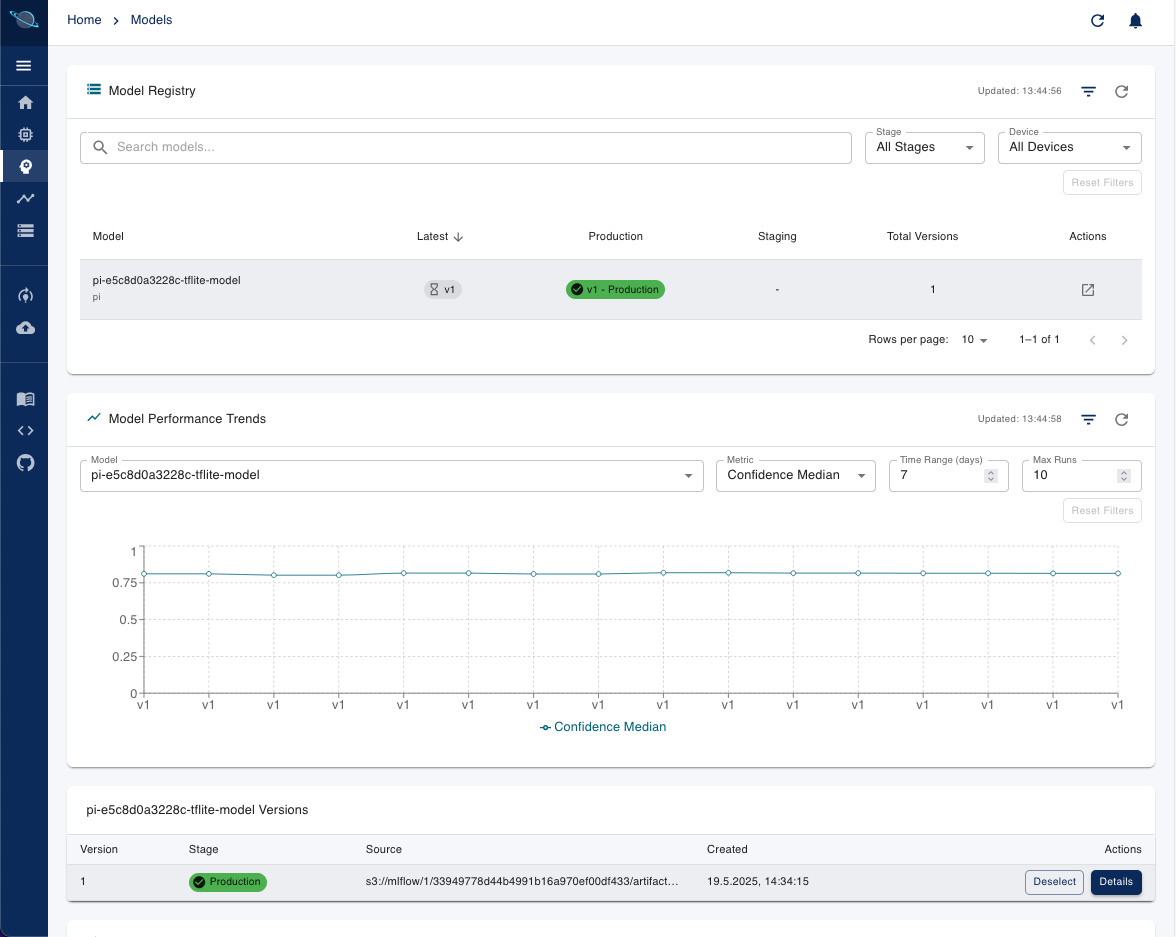
\includegraphics[width=\textwidth]{figs/framework/model-page.png}
        \caption{Model registry interface in TinySphere, listing available \gls{ml} models, their versions, and associated metadata for management.}
        \label{fig:ui_model_registry}
    \end{subfigure}

    \vspace{1em}

    \begin{subfigure}[b]{0.48\textwidth}
        \centering
        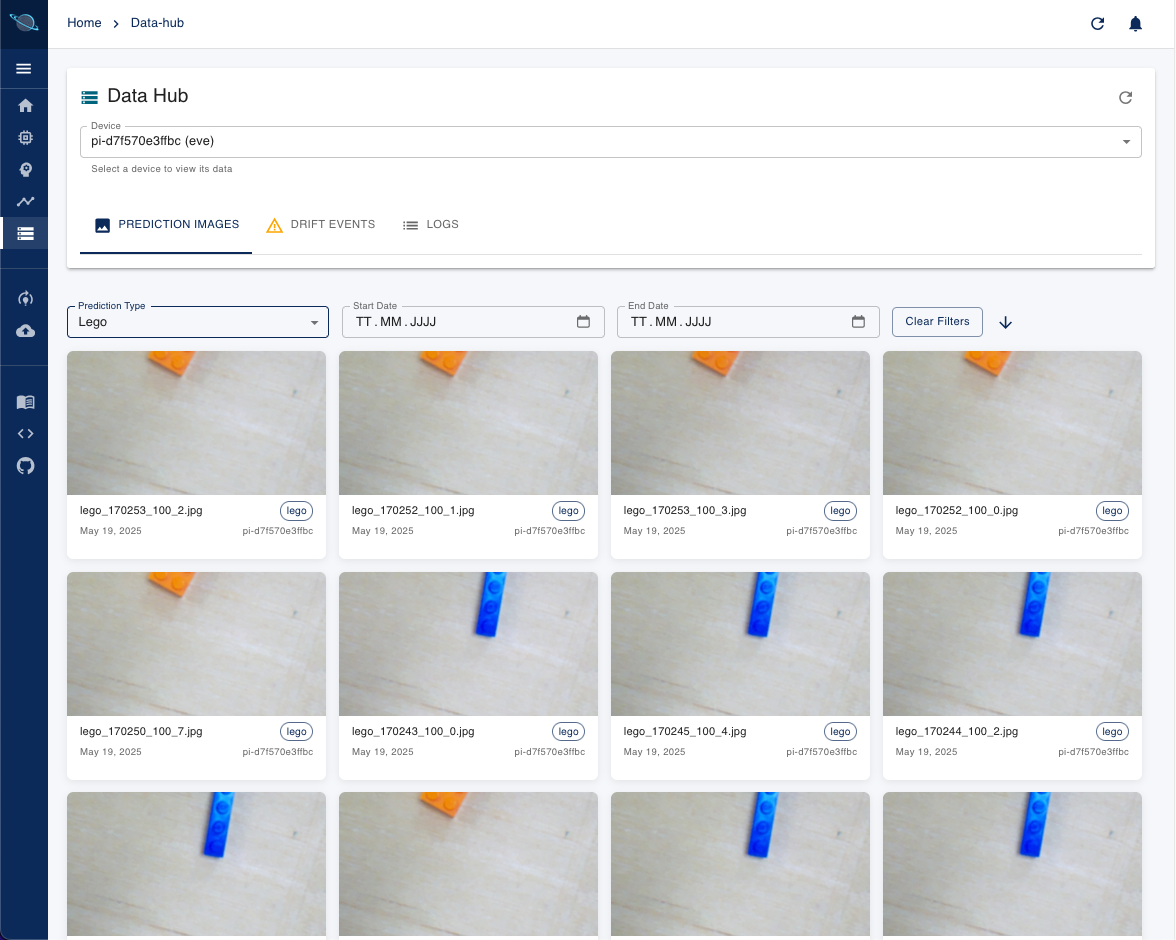
\includegraphics[width=\textwidth]{figs/framework/data-hub-page.png}
        \caption{Data Hub view in TinySphere, illustrating the aggregation and accessibility of data collected from deployed \gls{tinylcm} devices.}
        \label{fig:ui_data_hub}
    \end{subfigure}
    \hfill
    \begin{subfigure}[b]{0.48\textwidth}
        \centering
        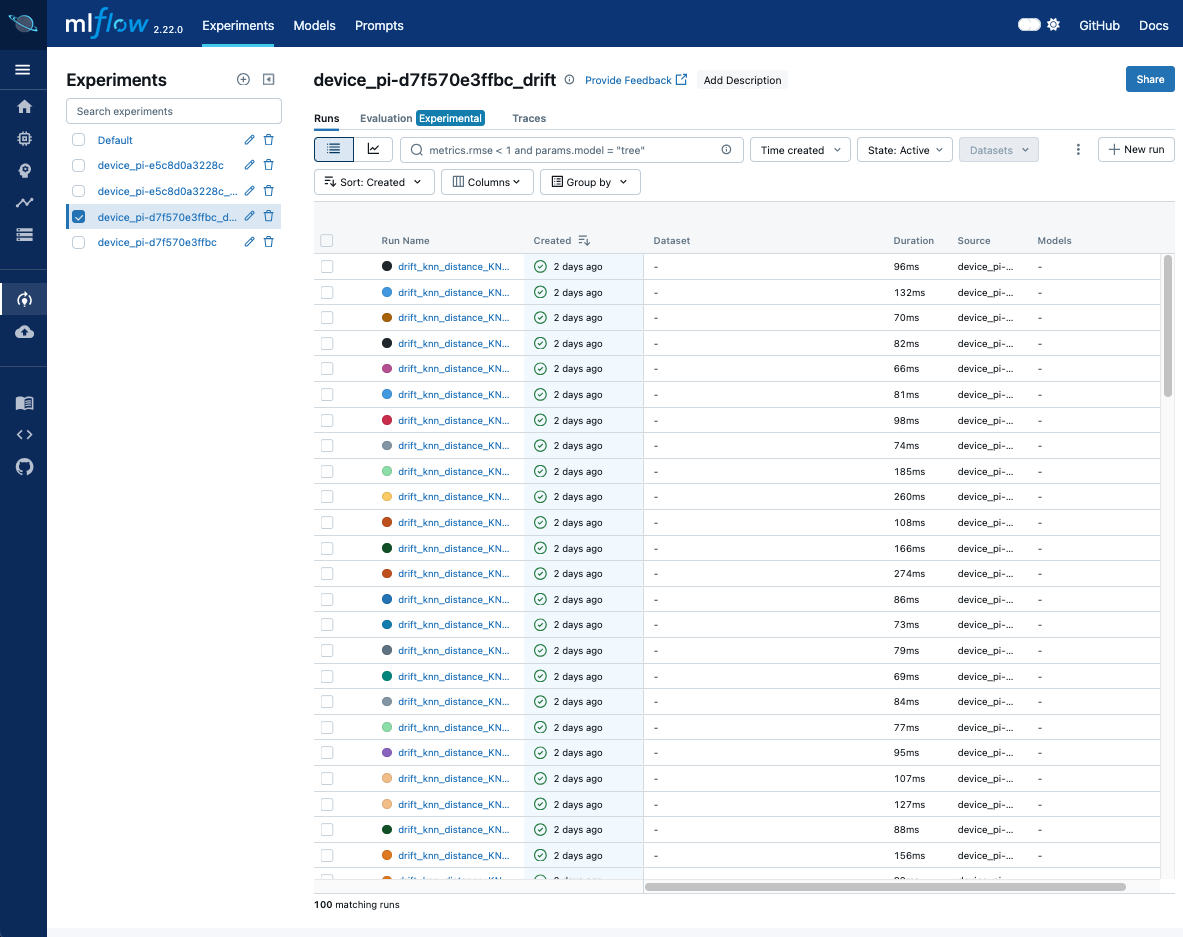
\includegraphics[width=\textwidth]{figs/framework/mlflow-page.png}
        \caption{Integration with MLflow, showcasing tracked experiments and runs, including logged parameters, metrics, and artifacts.}
        \label{fig:ui_mlflow_integration}
    \end{subfigure}

    \vspace{1em}
    \begin{subfigure}[b]{0.48\textwidth}
        \centering
        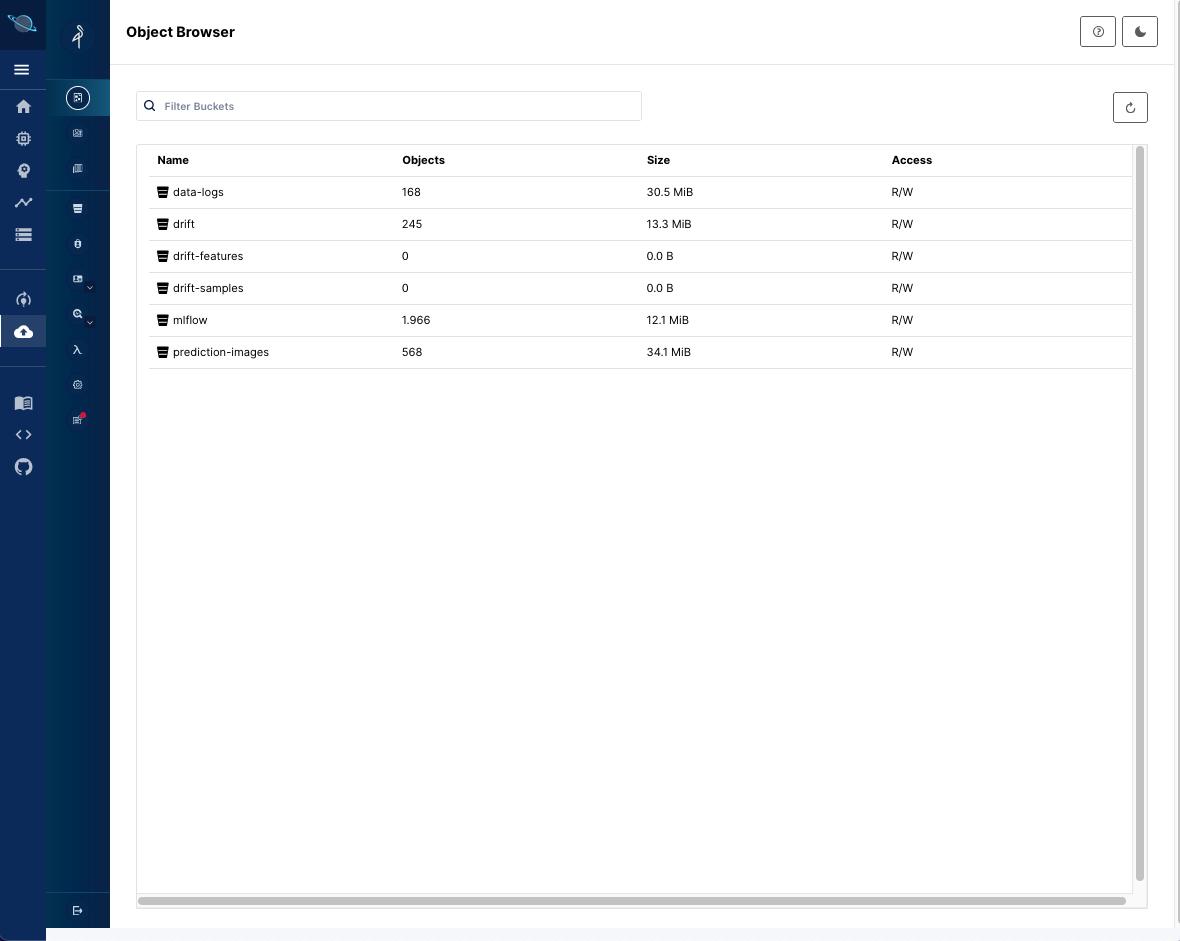
\includegraphics[width=\textwidth]{figs/framework/minio-page.png}
        \caption{MinIO object storage integration, displaying the bucket structure used for storing artifacts such as models, datasets, and logs.}
        \label{fig:ui_minio_integration}
    \end{subfigure}
    \hfill
    \begin{subfigure}[b]{0.48\textwidth}
        \centering
        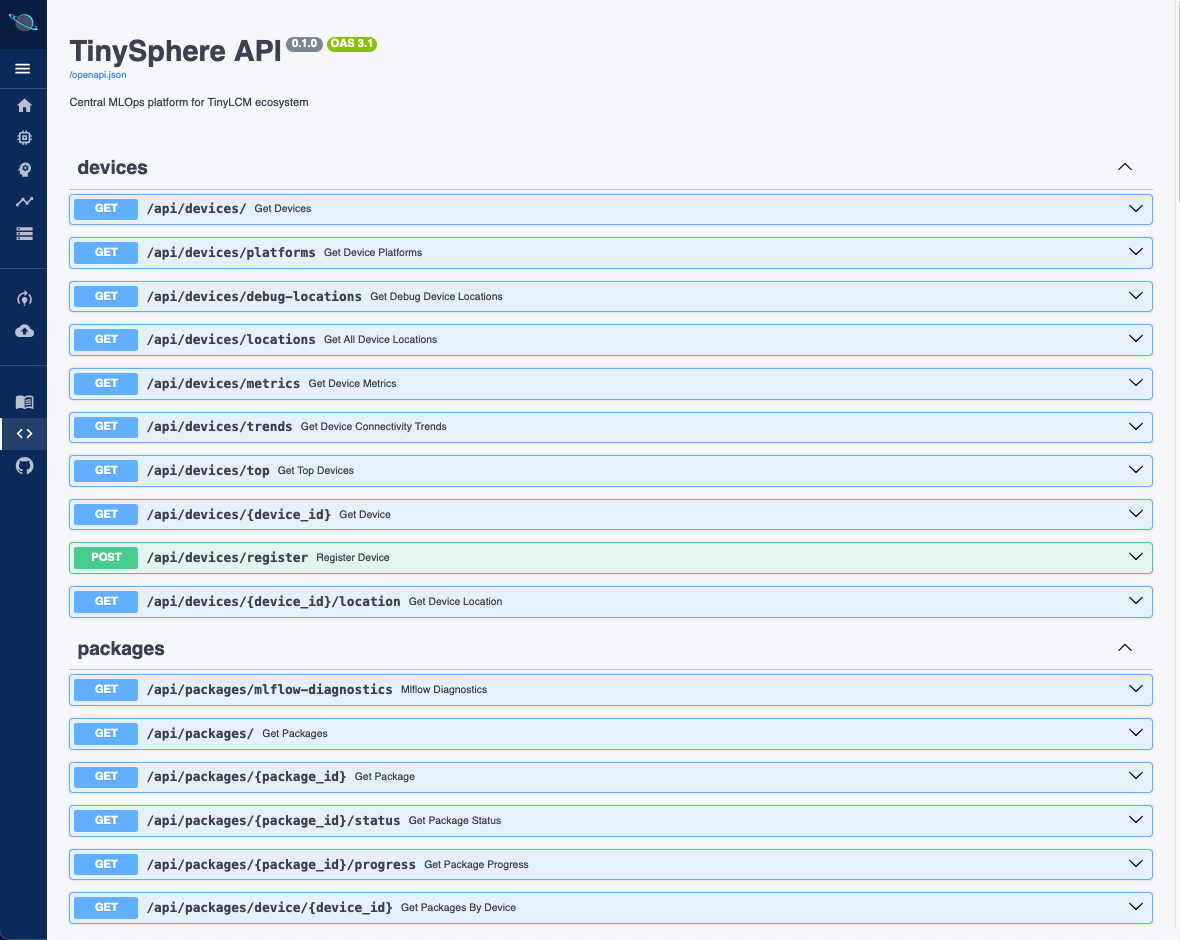
\includegraphics[width=\textwidth]{figs/framework/api-page.png}
        \caption{Integrated OpenAPI (Swagger) documentation for the TinySphere API, providing an interactive reference for developers.}
        \label{fig:ui_openapi_docs}
    \end{subfigure}

    \caption[Illustrative mockups of TinySphere User Interface components]{Illustrative mockups of TinySphere User Interface components and integrations supporting the MLOps workflow: (a) Device fleet management page, (b) Model registry, (c) Data Hub, (d) MLflow experiment tracking, (e) MinIO bucket structure, and (f) OpenAPI documentation.}
    \label{fig:tinysphere_ui_examples}
\end{figure}
